\paperchapter{September 2016}{25 September 2016}{A}{60}{GSET 2016}
\keytable{\kcell{1}{B} & \kcell{2}{A} & \kcell{3}{D} & \kcell{4}{C} & \kcell{5}{A} & \kcell{6}{B} & \kcell{7}{C} & \kcell{8}{C} & \kcell{9}{C} & \kcell{10}{B} \\
\kcell{11}{C} & \kcell{12}{D} & \kcell{13}{A} & \kcell{14}{A} & \kcell{15}{D} & \kcell{16}{C} & \kcell{17}{C} & \kcell{18}{C} & \kcell{19}{C} & \kcell{20}{B} \\
\kcell{21}{D} & \kcell{22}{A} & \kcell{23}{A} & \kcell{24}{B} & \kcell{25}{D} & \kcell{26}{B} & \kcell{27}{A} & \kcell{28}{C} & \kcell{29}{A} & \kcell{30}{B} \\
\kcell{31}{A} & \kcell{32}{A} & \kcell{33}{C} & \kcell{34}{B} & \kcell{35}{C} & \kcell{36}{C} & \kcell{37}{A} & \kcell{38}{B} & \kcell{39}{B} & \kcell{40}{C} \\
\kcell{41}{B} & \kcell{42}{C} & \kcell{43}{C} & \kcell{44}{C} & \kcell{45}{B} & \kcell{46}{C} & \kcell{47}{C} & \kcell{48}{B} & \kcell{49}{A} & \kcell{50}{B} \\
\kcell{51}{C} & \kcell{52}{A} & \kcell{53}{C} & \kcell{54}{C} & \kcell{55}{C} & \kcell{56}{D} & \kcell{57}{A} & \kcell{58}{C} & \kcell{59}{B} & \kcell{60}{A}}
\begin{question}{1}
{The purpose of evaluation is:\par}
\optstwo{Observation}{Decision-making}{Revision}{Review}
\answer{B}{Decision-making}
\begin{explain}
Evaluation collects evidence about learning in order to make judgements and \textbf{take decisions}: about promotion, selection, remedial teaching, improvement of methods and curriculum, and so on. Evaluation is essentially a \emph{decision-making} process.
\end{explain}
\end{question}

\begin{question}{2}
{What is the most essential factor for success of students learning?\par}
\optstwo{Readiness of learner}{Teacher's teaching}{Difficulty of content}{Classroom interaction}
\answer{A}{Readiness of learner}
\begin{explain}
\textbf{Readiness} of the learner is the foremost condition of learning. It covers physical, mental, emotional and motivational preparedness (Thorndike's \emph{Law of Readiness}). Without it, even the best teaching does not produce learning.
\end{explain}
\end{question}

\begin{question}{3}
{The student who keeps on asking questions in the class:\par}
\optsone{Should be advised to meet teacher personally}{Should be encouraged to participate in classroom discussion}{Should be encouraged for self learning}{Should be encouraged for continue questioning}
\answer{D}{Should be encouraged for continue questioning}
\begin{explain}
A student's questions show curiosity and active thinking. A good teacher \textbf{encourages continued questioning}, which sustains inquiry and critical thinking, and answers patiently rather than suppressing or diverting the student.
\end{explain}
\end{question}

\begin{question}{4}
{Heuristic is a method in which:\par}
\optsone{The teacher leads an inquiry}{ICT plays an important role}{The students strive to find out the solution}{Teaching of values is emphasised}
\answer{C}{The students strive to find out the solution}
\begin{explain}
In the \textbf{heuristic method} (H.~E.~Armstrong; Greek \emph{heurisko}, ``I discover'') the students themselves \textbf{strive to find out the solution}, behaving like discoverers. The teacher only guides.
\end{explain}
\end{question}

\begin{question}{5}
{Effective learning means:\par}
\optsone{Modification in behaviour of learner}{Consistency in behaviour of learner}{To recall information by the learner}{Good performance of learner in examination}
\answer{A}{Modification in behaviour of learner}
\begin{explain}
Learning is defined as a relatively permanent \textbf{modification of behaviour} resulting from experience. Effective learning brings desirable change in the learner's knowledge, skills and attitudes, not merely recall or examination scores.
\end{explain}
\end{question}

\begin{question}{6}
{Which is the most appropriate maxim for deductive method?\par}
\optstwo{Specific to General}{General to Specific}{Analytical to Integrative}{Known to Unknown}
\answer{B}{General to Specific}
\begin{explain}
Deduction moves from \textbf{general to specific}: a rule or principle is stated first and then applied to particular examples. Induction moves from specific to general.
\end{explain}
\end{question}

\begin{question}{7}
{If the purpose of the research is for theory building, then it is a:\par}
\optstwo{Action Research}{Historical Research}{Fundamental Research}{Applied Research}
\answer{C}{Fundamental Research}
\begin{explain}
\textbf{Fundamental (basic or pure) research} aims at extending knowledge and \textbf{building or testing theory}, without regard to immediate practical application.
\why{Action research solves immediate local problems; applied research solves practical problems; historical research studies the past.}
\end{explain}
\end{question}

\begin{question}{8}
{The list of titles-books, research reports, articles, papers etc., that may or may not have been referred to in the text of the research report is known as:\par}
\optsfour{References}{Footnotes}{Bibliography}{Appendices}
\answer{C}{Bibliography}
\begin{explain}
A \textbf{bibliography} lists all the sources consulted for the research, \emph{whether or not} they are cited in the text. \emph{References} include only the works actually cited.
\end{explain}
\end{question}

\begin{question}{9}
{Identify the unethical practice of a researcher from the following:\par}
\optstwo{Avoiding Plagiarism}{Avoiding Duplication}{Avoiding Reliable Information}{Avoiding Manipulation}
\answer{C}{Avoiding Reliable Information}
\begin{explain}
Every option except (C) describes an ethical practice. \textbf{Avoiding reliable information}, i.e.\ deliberately ignoring or suppressing trustworthy data, is unethical because it biases the findings.
\end{explain}
\end{question}

\begin{question}{10}
{Snowball sampling technique is a:\par}
\optsone{Probability sampling technique}{Non-probability sampling technique}{Both Probability and Non-probability sampling technique}{Not a sampling technique}
\answer{B}{Non-probability sampling technique}
\begin{explain}
\textbf{Snowball sampling} is a \textbf{non-probability} technique: each participant refers further participants from their own network. It is used for hidden or hard-to-reach populations.
\end{explain}
\end{question}

\begin{question}{11}
{In order to understand the classroom teaching-learning process, which of the following research tool is most appropriate?\par}
\optstwo{Rating Scale}{Questionnaire}{Observation Schedule}{Interview Schedule}
\answer{C}{Observation Schedule}
\begin{explain}
To study the actual classroom teaching--learning \emph{process}, the researcher must observe it directly as it happens, using an \textbf{observation schedule} (e.g.\ Flanders' Interaction Analysis Categories).
\end{explain}
\end{question}

\begin{question}{12}
{A hypothesis that states zero difference or no difference between the parameter and its assumed value is known as:\par}
\optstwo{Simple hypothesis}{Directional hypothesis}{Non-directional hypothesis}{Null hypothesis}
\answer{D}{Null hypothesis}
\begin{explain}
The \textbf{null hypothesis} ($H_0$) states \textbf{no difference} or no relationship, e.g.\ $\mu=\mu_0$ or $\mu_1=\mu_2$. It is the hypothesis that statistical tests evaluate.
\end{explain}
\end{question}

\begin{context}
\textbf{Read the paragraph and answer the Question Nos.~13--18.}\par\smallskip
Far from being a stern and severe intellectual remote from the world, Dr.~Radhakrishnan was a very humane person. Exceedingly popular among his students right from his early days as a professor at Presidency College, Madras he was an evocative teacher. He was offered the professorship in Calcutta University when he was less than 30 years old. He served as Vice-Chancellor of Andhra University from 1931--1936. In 1939 he was appointed the Vice-Chancellor of Banaras Hindu University. Two year later he took over the Sir Sayaji Rao chair of Indian culture and civilization in Banaras.

His mastery on his subject and his clearity of thought and expression made him even much sought after teacher. But what made him even more popular was his warmhearteness and his ability to draw out people. This aspect of his personality continued to win him countless admires throughout his long and illustrious life.

In the last decades of British rule he was the most sophisticated and exalted analysis of Gandhi's work and thought and in free India he provided the ideological armour for Nehru's foreign policy.
\end{context}
\begin{question}{13}
{Find synonym of `Armour':\par}
\optsfour{Shield}{Weapon}{Dress}{Stick}
\answer{A}{Shield}
\begin{explain}
\textbf{Armour} is protective covering, i.e.\ a \textbf{shield}. (In the passage, Radhakrishnan provided the ``ideological armour'', the intellectual defence, for Nehru's foreign policy.)
\end{explain}
\end{question}

\begin{question}{14}
{His role during last decades of British rule was:\par}
\optstwo{Analysed and exalted Gandhiji's work}{Helped Nehruji}{Encouraged students}{Did meeting with educationalists}
\answer{A}{Analysed and exalted Gandhiji's work}
\begin{explain}
``In the last decades of British rule he was the most sophisticated and exalted \textbf{analysis of Gandhi's work} and thought.''
\end{explain}
\end{question}

\begin{question}{15}
{Antonym of Humane is:\par}
\optsfour{Reasonable}{Kind}{Rational}{Brutal}
\answer{D}{Brutal}
\begin{explain}
\textbf{Humane} means kind and compassionate; its antonym is \textbf{brutal} (cruel).
\end{explain}
\end{question}

\begin{question}{16}
{Which quality of Radhakrishnan made him more popular in public life?\par}
\optstwo{Extraordinary Talent}{Personality}{Warmheartedness}{Intelligence}
\answer{C}{Warmheartedness}
\begin{explain}
``But what made him even more popular was his \textbf{warmheartedness} and his ability to draw out people.''
\end{explain}
\end{question}

\begin{question}{17}
{From which college he started his career?\par}
\optstwo{Calcutta University}{Banaras Hindu University}{Presidency College, Madras}{Delhi University}
\answer{C}{Presidency College, Madras}
\begin{explain}
``Exceedingly popular among his students right from his early days as a professor at \textbf{Presidency College, Madras}.''
\end{explain}
\end{question}

\begin{question}{18}
{In which year he was appointed as Vice-Chancellor in Banaras Hindu University?\par}
\optsfour{1931}{1936}{1939}{1942}
\answer{C}{1939}
\begin{explain}
``In \textbf{1939} he was appointed the Vice-Chancellor of Banaras Hindu University.''
\end{explain}
\end{question}

\begin{question}{19}
{`Extemporaneous method' is a method of:\par}
\optsfour{Listening}{Reading}{Speaking}{Writing}
\answer{C}{Speaking}
\begin{explain}
\textbf{Extempore (extemporaneous) speaking} is a method of \textbf{speaking}: delivering a speech with little preparation, from brief notes rather than a written text.
\end{explain}
\end{question}

\begin{question}{20}
{The basic purpose of communication is:\par}
\optsfour{to Confirm}{to Inform}{to Reform}{to Form}
\answer{B}{to Inform}
\begin{explain}
The basic purpose of communication is \textbf{to inform}, i.e.\ to share information, ideas and feelings. Persuading, motivating and entertaining are further purposes built on this.
\end{explain}
\end{question}

\begin{question}{21}
{The competency of an effective communicator can be judged on the basis of:\par}
\optstwo{Personality of Communicator}{Interactivity with the target audience}{Experience in the field}{Meeting the needs of target audience}
\answer{D}{Meeting the needs of target audience}
\begin{explain}
A communicator is effective to the extent that the message \textbf{meets the needs of the target audience}: it is understood, accepted and acted upon. Personality, interactivity and experience help, but success is judged by the audience's needs being met.
\end{explain}
\end{question}

\begin{question}{22}
{The person who transmits the message is called the:\par}
\optsfour{Sender}{Receiver}{Barrier}{Decoder}
\answer{A}{Sender}
\begin{explain}
The person who originates and transmits the message is the \textbf{sender} (source or encoder).
\end{explain}
\end{question}

\begin{question}{23}
{Which of the following is required as a skill while reading?\par}
\optstwo{Ability to comprehend}{Reason for reading}{Time for reading}{Help in reading}
\answer{A}{Ability to comprehend}
\begin{explain}
The essential reading skill is the \textbf{ability to comprehend}, i.e.\ to understand and interpret the meaning of the text.
\end{explain}
\end{question}

\begin{question}{24}
{When reading the text only for relevant and required information is called:\par}
\optsfour{Skimming}{Scanning}{Reading}{Reviewing}
\answer{B}{Scanning}
\begin{explain}
\textbf{Scanning} is reading quickly to locate \emph{specific, required information} (a name, date or figure). \textbf{Skimming} is reading quickly to get the general idea or gist.
\end{explain}
\end{question}

\begin{question}{25}
{One number in the following number series is wrong. Find out the wrong number:\newline 196, 169, 144, 121, 101\par}
\optsfour{121}{169}{196}{101}
\answer{D}{101}
\begin{explain}
The series consists of squares of consecutive numbers in descending order: $14^2=196$, $13^2=169$, $12^2=144$, $11^2=121$, $10^2=\mathbf{100}$. So \textbf{101} is wrong.
\end{explain}
\end{question}

\begin{question}{26}
{The following series contains various terms of an alphabet series with one or more terms missing as shown by ? Choose the missing terms out of the given alternatives:\newline T, R, P, N, L, ?, ?\par}
\optsfour{J, G}{J, H}{K, H}{K, I}
\answer{B}{J, H}
\begin{explain}
Each letter moves two steps back: T, R, P, N, L, \textbf{J}, \textbf{H}.
\end{explain}
\end{question}

\begin{question}{27}
{Find out the next term in the coded series:\newline Z1A, X2D, V6G, T21J, R88M, P445P\par}
\optsfour{N2676S}{N2676T}{T2670N}{T2676N}
\answer{A}{N2676S}
\begin{explain}
\begin{itemize}
\item First letters: Z, X, V, T, R, P, \textbf{N} ($-2$).
\item Numbers: $1\times1+1=2$, $2\times2+2=6$, $6\times3+3=21$, $21\times4+4=88$, $88\times5+5=445$, $445\times6+6=\mathbf{2676}$.
\item Last letters: A, D, G, J, M, P, \textbf{S} ($+3$).
\end{itemize}
The next term is \textbf{N2676S}.
\end{explain}
\end{question}

\begin{question}{28}
{Pointing towards a person, a man said to a woman, "his mother is the only daughter of your father." How is woman related to that person?\par}
\optsfour{Daughter}{Sister}{Mother}{Wife}
\answer{C}{Mother}
\begin{explain}
``The only daughter of your father'' is the woman herself. So the person's mother is the woman, and the woman is the person's \textbf{mother}.
\end{explain}
\end{question}

\begin{question}{29}
{Choose the word which is least like the other words in the group:\par}
\optsfour{Flute}{Gitar}{Sitar}{Violin}
\answer{A}{Flute}
\begin{explain}
Guitar, sitar and violin are \textbf{string} instruments; the \textbf{flute} is a wind instrument.
\end{explain}
\end{question}

\begin{question}{30}
{If GOLD is coded as HOME, COME is coded as DONE and CORD is coded as DOSE, how would you code SONS?\par}
\optsfour{TPOT}{TOOT}{TOOS}{TONT}
\answer{B}{TOOT}
\begin{explain}
Pattern: 1st letter $+1$, 2nd letter unchanged, 3rd letter $+1$, 4th letter $+1$ (GOLD $\rightarrow$ HOME, COME $\rightarrow$ DONE, CORD $\rightarrow$ DOSE).
SONS $\rightarrow$ S$+1$, O, N$+1$, S$+1$ $=$ \textbf{TOOT}.
\end{explain}
\end{question}

\begin{question}{31}
{Konkani is related to Goa in the same way, Dogri is related to:\par}
\optstwo{Himachal Pradesh}{Sikkim}{Assam}{West Bengal}
\answer{A}{Himachal Pradesh}
\begin{explain}
\textbf{Konkani} is the official language of Goa. \textbf{Dogri} is spoken mainly in the Jammu region and in adjoining parts of \textbf{Himachal Pradesh}; among the options given, it is related to Himachal Pradesh. (Dogri was added to the Eighth Schedule by the 92nd Amendment, 2003.)
\end{explain}
\end{question}

\begin{question}{32}
{In the question below is given a statement followed by two assumptions numbered I and II.\newline Statement: Use of cell phones is not allowed inside auditorium.\newline Assumption I: All those who have cell phone will switch it off before they take their seats in the auditorium.\newline Assumption II: Generally people do not bring cell phones when they come to attend functions in the auditorium.\par}
\optstwo{Only assumption I is correct}{Only assumption II is correct}{Either I or II assumption is correct}{Neither I nor II assumption is correct}
\answer{A}{Only assumption I is correct}
\begin{explain}
The official key gives \textbf{only assumption I}. A rule prohibiting cell phones assumes that people \emph{will comply}, switching their phones off before taking their seats. Assumption II contradicts the need for the rule: if people did not bring phones, no prohibition would be needed.
\end{explain}
\end{question}

\begin{question}{33}
{Should there be a complete ban on Indian professionals seeking jobs elsewhere after getting their education in India?\newline Arguments:\newline I: Yes -- this is the only way to sustain the present rate of technological development in India.\newline II: No -- the Indians settled abroad send huge amount of foreign exchange and this constitutes significant part of foreign exchange reserve.\newline III: No -- the practical knowledge gained by Indians working in the other country help India develop its economy.\par}
\optsone{None is strong statement}{All the statements I, II and III are strong}{Only I and II are strong}{Only III is strong}
\answer{C}{Only I and II are strong}
\begin{explain}
The official key gives \textbf{only I and II are strong}. Argument I argues from the need to retain talent for India's technological development. Argument II points to the large foreign-exchange remittances from Indians abroad. Argument III is a weaker, general claim, according to the key.
\end{explain}
\end{question}

\begin{question}{34}
{The words: stationery, paper and ink are related. The relationship among these can best represented by which of the following diagrams?\par}
\optsfour{\tikz[baseline=-0.5ex,scale=0.3]{\draw (0,0) circle(1.2); \draw (0,0.2) circle(0.55);}}{\tikz[baseline=-0.5ex,scale=0.3]{\draw (0,0) circle(1.3); \draw (-0.55,0) circle(0.5); \draw (0.55,0) circle(0.5);}}{\tikz[baseline=-0.5ex,scale=0.3]{\draw (0,0) circle(1.3); \draw (-0.35,0) circle(0.6); \draw (0.35,0) circle(0.6);}}{\tikz[baseline=-0.5ex,scale=0.3]{\draw (0,0) circle(0.8); \draw (1.1,0) circle(0.8); \draw (2.2,0) circle(0.8);}}
\answer{B}{\tikz[baseline=-0.5ex,scale=0.3]{\draw (0,0) circle(1.3); \draw (-0.55,0) circle(0.5); \draw (0.55,0) circle(0.5);}}
\begin{explain}
Paper and ink are both items of \textbf{stationery}, but they are completely different things (no paper is ink). They are two \textbf{separate circles inside} the stationery circle, as in diagram (B).
\end{explain}
\end{question}

\begin{question}{35}
{Find the missing number in the following:\par}
\qfigure{\begin{tabular}{|c|c|c|}\hline 1 & 2 & 3\\\hline 4 & 5 & 6\\\hline 7 & 8 & 9\\\hline 27 & 38 & ?\\\hline\end{tabular}}
\optsfour{49}{50}{51}{52}
\answer{C}{51}
\begin{explain}
In each column, bottom $=$ (middle $\times$ third) $-$ top:
\[4\times7-1=27,\qquad 5\times8-2=38,\qquad 6\times9-3=\mathbf{51}\]
\end{explain}
\end{question}

\begin{question}{36}
{Count the number of triangles and squares in the following figure:\par}
\qfigure{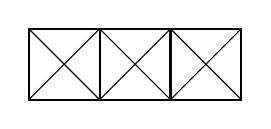
\begin{tikzpicture}[scale=0.9]
\foreach \x in {0,1,2} {\draw[thick] (\x,0) rectangle (\x+1,1); \draw (\x,0)--(\x+1,1); \draw (\x,1)--(\x+1,0);}
\end{tikzpicture}}
\optstwo{28 triangles, 3 squares}{24 triangles, 5 squares}{28 triangles, 5 squares}{24 triangles, 3 squares}
\answer{C}{28 triangles, 5 squares}
\begin{explain}
\textbf{Triangles.} Each square with both diagonals contains 4 small triangles and 4 half-square triangles, i.e.\ $8\times3=24$. Across each pair of adjacent squares, the diagonals meeting at the shared top (or bottom) corner form a larger triangle on the base of two squares: $2$ pairs $\times$ $2$ (top and bottom) $=4$. Total $=\mathbf{28}$.

\textbf{Squares.} There are 3 visible squares. Around each shared vertical edge, the diagonals of the two neighbouring squares form a tilted square (a diamond), which adds 2 more. Total $=\mathbf{5}$.
\end{explain}
\end{question}

\begin{question}{37}
{`CENSUS' data are:\par}
\optstwo{Primary data}{Secondary data}{Simulated data}{Cross-sectional data}
\answer{A}{Primary data}
\begin{explain}
The official key treats \textbf{census data as primary data}: they are collected directly, first-hand, from every unit of the population by the census organisation. (For other researchers who later use published census tables, the same data become secondary data.)
\end{explain}
\end{question}

\begin{question}{38}
{The data collected on various blood groups of a population of a city is:\par}
\optstwo{Quantitative data}{Qualitative data}{Continuous data}{Descriptive data}
\answer{B}{Qualitative data}
\begin{explain}
Blood groups (A, B, AB, O) are \textbf{categories}, not measurements, so they are \textbf{qualitative (nominal)} data.
\end{explain}
\end{question}

\begin{question}{39}
{The following pie diagram shows the amounts that a family spends on: Food, clothing, rent and miscellaneous expenditure and savings. If the monthly income of the family is 60,000, then monthly savings are:\par}
\qfigure{\begin{tikzpicture}\pie[radius=1.4,text=pin,font=\scriptsize,hide number,color={brand!25,brand!10,brand!35,brand!15,brand!5}]{30/Food 108\textdegree,20/Rent 72\textdegree,20/Clothing 72\textdegree,20/Misc.\ 72\textdegree,10/Savings}\end{tikzpicture}}
\optsfour{3,000}{6,000}{7,500}{9,000}
\answer{B}{6,000}
\begin{explain}
Savings $=360^\circ-(108+72+72+72)^\circ=36^\circ$.
\[\text{Savings}=\frac{36}{360}\times60{,}000=\mathbf{6{,}000}\]
\end{explain}
\end{question}

\begin{question}{40}
{The following bar diagram shows the registration of CARS and total vehicles during the first six months of the year 2004 in DELHI:\par}
\qfigure{\begin{tikzpicture}
\begin{axis}[ybar,width=10cm,height=4.4cm,bar width=9pt,ymin=0,ymax=52,
  symbolic x coords={Jan,Feb,Mar,Apr,May,Jun},xtick=data,legend style={font=\tiny,at={(1.02,1)},anchor=north west},
  nodes near coords,every node near coord/.append style={font=\tiny},tick label style={font=\scriptsize},
  ylabel={\scriptsize Registrations ('000)},axis x line*=bottom,axis y line*=left]
\addplot[fill=white,draw=ink] coordinates {(Jan,21) (Feb,15) (Mar,22) (Apr,20) (May,17) (Jun,28)};
\addplot[pattern=north east lines,draw=ink] coordinates {(Jan,27) (Feb,22) (Mar,25) (Apr,35) (May,35) (Jun,45)};
\legend{Cars,Total vehicles}
\end{axis}
\end{tikzpicture}}
What was the percentage increase in registration of CARS from MAY to JUNE 2004?
\optsfour{64.2\%}{64.5\%}{64.7\%}{64.9\%}
\answer{C}{64.7\%}
\begin{explain}
Cars: May $=17$ thousand, June $=28$ thousand.
\[\frac{28-17}{17}\times100=\frac{11}{17}\times100\approx\mathbf{64.7\%}\]
\end{explain}
\end{question}

\begin{question}{41}
{The number of male and female students registered for their Ph.D. programme in various faculties along with their total strength in years 2006-2015 can be `best' represented by a:\par}
\optstwo{Simple bar diagram}{Multiple bar diagram}{Histogram}{Pie diagram}
\answer{B}{Multiple bar diagram}
\begin{explain}
The data show male and female numbers (and totals) for each faculty over several years, i.e.\ several related quantities side by side for each category. A \textbf{multiple (grouped) bar diagram} represents this best.
\why{A simple bar diagram shows one variable; a histogram is for continuous frequency distributions; a pie diagram shows the parts of one whole.}
\end{explain}
\end{question}

\begin{question}{42}
{Raw data collected on: height, weight, BMI and age can be:\par}
\optstwo{classified}{tabulated}{both classified and tabulated}{categorized}
\answer{C}{both classified and tabulated}
\begin{explain}
Raw data on height, weight, BMI and age can first be \textbf{classified} (grouped into classes) and then \textbf{tabulated} (arranged in rows and columns) for analysis.
\end{explain}
\end{question}

\begin{question}{43}
{Which of the following is the Web browser?\par}
\optsfour{Windows 7}{C++ Language}{Google Chrome}{Tally}
\answer{C}{Google Chrome}
\begin{explain}
\textbf{Google Chrome} is a web browser.
\why{Windows 7 is an operating system, C++ is a programming language, and Tally is accounting software.}
\end{explain}
\end{question}

\begin{question}{44}
{What is the full form of MOOC?\par}
\optstwo{Most Organised Offline Courses}{Modern Online Office Courses}{Massive Open Online Courses}{Massive Office Order Cell}
\answer{C}{Massive Open Online Courses}
\begin{explain}
\textbf{MOOC} is \textbf{Massive Open Online Course}, an online course open to unlimited participants (e.g.\ SWAYAM, Coursera, edX).
\end{explain}
\end{question}

\begin{question}{45}
{Which number system is used to store data and perform calculation in computers?\par}
\optsfour{Octal}{Binary}{Decimal}{Hexadecimal}
\answer{B}{Binary}
\begin{explain}
Computers store data and compute in the \textbf{binary} number system (0 and 1), matching the two states of electronic circuits.
\end{explain}
\end{question}

\begin{question}{46}
{Which law protects the crimes through Internet?\par}
\optsfour{IT Law}{Common Law}{Cyber Law}{Natural Law}
\answer{C}{Cyber Law}
\begin{explain}
Crimes committed through computers and the Internet are dealt with by \textbf{cyber law}. In India this is chiefly the Information Technology Act, 2000 (amended in 2008).
\end{explain}
\end{question}

\begin{question}{47}
{ATM stands for:\par}
\optstwo{All Time Money}{Auto Teller Machine}{Automated Teller Machine}{Arithmetic Teller Machine}
\answer{C}{Automated Teller Machine}
\begin{explain}
\textbf{ATM} is \textbf{Automated Teller Machine}.
\end{explain}
\end{question}

\begin{question}{48}
{Personal data is often transmitted over the internet. One method of securing the data before transmission is:\par}
\optstwo{Filtering}{Using encryption}{Using firewall}{Streaming}
\answer{B}{Using encryption}
\begin{explain}
\textbf{Encryption} converts data into a coded (cipher) form that only authorised parties with the key can read, e.g.\ SSL/TLS (HTTPS). This secures personal data in transit.
\end{explain}
\end{question}

\begin{question}{49}
{Chemistry of corrosion is:\par}
\optstwo{Electrochemical Phenomenon}{Physiochemical Phenomenon}{Reduction}{Hydrothermal Reaction}
\answer{A}{Electrochemical Phenomenon}
\begin{explain}
Corrosion (e.g.\ rusting of iron) is an \textbf{electrochemical} process. Anodic and cathodic regions form on the metal surface, with oxidation $\mathrm{Fe}\rightarrow\mathrm{Fe}^{2+}+2e^-$ and reduction of oxygen, and moisture acts as the electrolyte.
\end{explain}
\end{question}

\begin{question}{50}
{Which is not correct for `green chemistry'?\par}
\optsone{Design benign chemicals}{Design for non-degradation}{Design to reduce the use and generation of hazardous substances}{Design for strategic pathway to build a sustainable future}
\answer{B}{Design for non-degradation}
\begin{explain}
The \emph{12 Principles of Green Chemistry} (Anastas \& Warner) include designing safer (benign) chemicals, reducing hazardous substances and \textbf{designing for degradation}: products should break down into harmless substances after use. ``Design for \emph{non}-degradation'' is therefore not correct.
\end{explain}
\end{question}

\begin{question}{51}
{The work of Hargobind Khorana in which he got Nobel Prize was:\par}
\optstwo{Penicillin}{Sulpha drug}{Cracking of genetic code}{Pairing of nucleotide base}
\answer{C}{Cracking of genetic code}
\begin{explain}
\textbf{Har Gobind Khorana} shared the 1968 Nobel Prize in Physiology or Medicine (with Nirenberg and Holley) for the \textbf{interpretation (cracking) of the genetic code} and its role in protein synthesis.
\end{explain}
\end{question}

\begin{question}{52}
{Amount of organic pollutants found in surface water is measured by:\par}
\optstwo{COD (Chemical Oxygen Demand)}{Energy efficient batteries}{3-D printed structure}{Gas sensitive semiconductor technology}
\answer{A}{COD (Chemical Oxygen Demand)}
\begin{explain}
\textbf{COD (Chemical Oxygen Demand)} measures the oxygen needed to chemically oxidise organic pollutants in water. It is an indicator of organic pollution (together with BOD).
\end{explain}
\end{question}

\begin{question}{53}
{Bubblegum contains:\par}
\optstwo{Natural Rubber}{Synthetic Rubber}{Synthetic Styrenebutadiene Rubber}{Styrene Maleic Anhydride}
\answer{C}{Synthetic Styrenebutadiene Rubber}
\begin{explain}
Chewing-gum and bubble-gum bases use synthetic elastomers, mainly \textbf{styrene--butadiene rubber (SBR)} and polyisobutylene, which give them stretch and elasticity.
\end{explain}
\end{question}

\begin{question}{54}
{To raise global awareness, which day every year we celebrate Environment Day?\par}
\optsfour{10th May}{13th March}{5th June}{17th January}
\answer{C}{5th June}
\begin{explain}
\textbf{World Environment Day} is celebrated on \textbf{5 June} every year (UNEP; first observed in 1974, commemorating the 1972 Stockholm Conference).
\end{explain}
\end{question}

\begin{question}{55}
{What is the main objective of NAAC in India?\par}
\optstwo{Establishing Universities}{Evaluating Universities}{Accrediting Universities}{Funding Universities}
\answer{C}{Accrediting Universities}
\begin{explain}
The main objective of \textbf{NAAC} is the \textbf{assessment and accreditation} of higher-education institutions.
\end{explain}
\end{question}

\begin{question}{56}
{"Gujarat Vidyapith", Ahmedabad is a:\par}
\optstwo{Central University}{State University}{Private University}{Deemed University}
\answer{D}{Deemed University}
\begin{explain}
\textbf{Gujarat Vidyapith}, founded by Mahatma Gandhi in 1920, is a \textbf{deemed university} (since 1963).
\end{explain}
\end{question}

\begin{question}{57}
{Which of the following is a popular programme for promoting science and technology supported by Department of Science and Technology (DST), Govt. of India?\par}
\optsfour{INSPIRE}{SCOPE}{PMOST}{SSA}
\answer{A}{INSPIRE}
\begin{explain}
\textbf{INSPIRE} (Innovation in Science Pursuit for Inspired Research, 2008) is DST's flagship programme to attract young talent to science through scholarships, fellowships and awards (e.g.\ INSPIRE-MANAK).
\end{explain}
\end{question}

\begin{question}{58}
{Which of the following is a Central University?\par}
\optstwo{Gujarat University}{Mohanlal Sukhadia University}{Banaras Hindu University}{Mumbai University}
\answer{C}{Banaras Hindu University}
\begin{explain}
\textbf{Banaras Hindu University} (founded 1916 by Madan Mohan Malaviya) is a central university.
\why{Gujarat University, Mohanlal Sukhadia University (Udaipur) and the University of Mumbai are state universities.}
\end{explain}
\end{question}

\begin{question}{59}
{Which of the following is an Exclusive Women University?\par}
\optstwo{University of Delhi}{SNDT University}{Gujarat Vidyapeeth}{Visva-Bharati University}
\answer{B}{SNDT University}
\begin{explain}
\textbf{SNDT Women's University}, Mumbai (founded 1916 by Dhondo Keshav Karve) is India's first exclusively women's university.
\end{explain}
\end{question}

\begin{question}{60}
{For which field the Vikram Sarabhai Awards are given?\par}
\optstwo{Biological Research}{Agricultural Research}{Space Research}{Mathematical Research}
\answer{A}{Biological Research}
\keynote{The official key gives (A). Students should note that the best-known \emph{Vikram Sarabhai Research Award} (Physical Research Laboratory) and the \emph{Vikram Sarabhai Memorial Award} (COSPAR) relate to space science. Answer as per the key in the exam context.}
\begin{explain}
Awards named after Dr.~Vikram Sarabhai, the father of India's space programme, are given in several fields of science. The official GSET key identifies the field as \textbf{biological research}.
\end{explain}
\end{question}
